% This is "sig-alternate.tex" V2.1 April 2013
% This file should be compiled with V2.5 of "sig-alternate.cls" May 2012
%
% This example file demonstrates the use of the 'sig-alternate.cls'
% V2.5 LaTeX2e document class file. It is for those submitting
% articles to ACM Conference Proceedings WHO DO NOT WISH TO
% STRICTLY ADHERE TO THE SIGS (PUBS-BOARD-ENDORSED) STYLE.
% The 'sig-alternate.cls' file will produce a similar-looking,
% albeit, 'tighter' paper resulting in, invariably, fewer pages.
%
% ----------------------------------------------------------------------------------------------------------------
% This .tex file (and associated .cls V2.5) produces:
%       1) The Permission Statement
%       2) The Conference (location) Info information
%       3) The Copyright Line with ACM data
%       4) NO page numbers
%
% as against the acm_proc_article-sp.cls file which
% DOES NOT produce 1) thru' 3) above.
%
% Using 'sig-alternate.cls' you have control, however, from within
% the source .tex file, over both the CopyrightYear
% (defaulted to 200X) and the ACM Copyright Data
% (defaulted to X-XXXXX-XX-X/XX/XX).
% e.g.
% \CopyrightYear{2007} will cause 2007 to appear in the copyright line.
% \crdata{0-12345-67-8/90/12} will cause 0-12345-67-8/90/12 to appear in the copyright line.
%
% ---------------------------------------------------------------------------------------------------------------
% This .tex source is an example which *does* use
% the .bib file (from which the .bbl file % is produced).
% REMEMBER HOWEVER: After having produced the .bbl file,
% and prior to final submission, you *NEED* to 'insert'
% your .bbl file into your source .tex file so as to provide
% ONE 'self-contained' source file.
%
% ================= IF YOU HAVE QUESTIONS =======================
% Questions regarding the SIGS styles, SIGS policies and
% procedures, Conferences etc. should be sent to
% Adrienne Griscti (griscti@acm.org)
%
% Technical questions _only_ to
% Gerald Murray (murray@hq.acm.org)
% ===============================================================
%
% For tracking purposes - this is V2.0 - May 2012

\documentclass{sig-alternate-05-2015}
\usepackage{subfigure} 

\begin{document}

% Copyright
\setcopyright{acmcopyright}
%\setcopyright{acmlicensed}
%\setcopyright{rightsretained}
%\setcopyright{usgov}
%\setcopyright{usgovmixed}
%\setcopyright{cagov}
%\setcopyright{cagovmixed}


% DOI
\doi{10.475/123_4}

% ISBN
\isbn{123-4567-24-567/08/06}

%Conference
\conferenceinfo{PLDI '13}{June 16--19, 2013, Seattle, WA, USA}

\acmPrice{\$15.00}

%
% --- Author Metadata here ---
\conferenceinfo{WOODSTOCK}{'97 El Paso, Texas USA}
%\CopyrightYear{2007} % Allows default copyright year (20XX) to be over-ridden - IF NEED BE.
%\crdata{0-12345-67-8/90/01}  % Allows default copyright data (0-89791-88-6/97/05) to be over-ridden - IF NEED BE.
% --- End of Author Metadata ---

\title{Will Docker Container Affect Latency
%\titlenote{(Produces the permission block, and
%copyright information). For use with
%SIG-ALTERNATE.CLS. Supported by ACM.}
}
%\subtitle{[Extended Abstract]
%\titlenote{A full version of this paper is available as
%\textit{Author's Guide to Preparing ACM SIG Proceedings Using
%\LaTeX$2_\epsilon$\ and BibTeX} at
%\texttt{www.acm.org/eaddress.htm}}}
%
% You need the command \numberofauthors to handle the 'placement
% and alignment' of the authors beneath the title.
%
% For aesthetic reasons, we recommend 'three authors at a time'
% i.e. three 'name/affiliation blocks' be placed beneath the title.
%
% NOTE: You are NOT restricted in how many 'rows' of
% "name/affiliations" may appear. We just ask that you restrict
% the number of 'columns' to three.
%
% Because of the available 'opening page real-estate'
% we ask you to refrain from putting more than six authors
% (two rows with three columns) beneath the article title.
% More than six makes the first-page appear very cluttered indeed.
%
% Use the \alignauthor commands to handle the names
% and affiliations for an 'aesthetic maximum' of six authors.
% Add names, affiliations, addresses for
% the seventh etc. author(s) as the argument for the
% \additionalauthors command.
% These 'additional authors' will be output/set for you
% without further effort on your part as the last section in
% the body of your article BEFORE References or any Appendices.

\numberofauthors{8} %  in this sample file, there are a *total*
% of EIGHT authors. SIX appear on the 'first-page' (for formatting
% reasons) and the remaining two appear in the \additionalauthors section.
%
\author{
% You can go ahead and credit any number of authors here,
% e.g. one 'row of three' or two rows (consisting of one row of three
% and a second row of one, two or three).
%
% The command \alignauthor (no curly braces needed) should
% precede each author name, affiliation/snail-mail address and
% e-mail address. Additionally, tag each line of
% affiliation/address with \affaddr, and tag the
% e-mail address with \email.
%
% 1st. author
\alignauthor
Ben Trovato\titlenote{Dr.~Trovato insisted his name be first.}\\
       \affaddr{Institute for Clarity in Documentation}\\
       \affaddr{1932 Wallamaloo Lane}\\
       \affaddr{Wallamaloo, New Zealand}\\
       \email{trovato@corporation.com}
% 2nd. author
\alignauthor
G.K.M. Tobin\titlenote{The secretary disavows
any knowledge of this author's actions.}\\
       \affaddr{Institute for Clarity in Documentation}\\
       \affaddr{P.O. Box 1212}\\
       \affaddr{Dublin, Ohio 43017-6221}\\
       \email{webmaster@marysville-ohio.com}
% 3rd. author
\alignauthor Lars Th{\o}rv{\"a}ld\titlenote{This author is the
one who did all the really hard work.}\\
       \affaddr{The Th{\o}rv{\"a}ld Group}\\
       \affaddr{1 Th{\o}rv{\"a}ld Circle}\\
       \affaddr{Hekla, Iceland}\\
       \email{larst@affiliation.org}
}
% There's nothing stopping you putting the seventh, eighth, etc.
% author on the opening page (as the 'third row') but we ask,
% for aesthetic reasons that you place these 'additional authors'
% in the \additional authors block, viz.
%\additionalauthors{Additional authors: John Smith (The Th{\o}rv{\"a}ld Group,
%email: {\texttt{jsmith@affiliation.org}}) and Julius P.~Kumquat
%(The Kumquat Consortium, email: {\texttt{jpkumquat@consortium.net}}).}
%\date{30 July 1999}
% Just remember to make sure that the TOTAL number of authors
% is the number that will appear on the first page PLUS the
% number that will appear in the \additionalauthors section.

\maketitle
\begin{abstract}
Traditionally, many web services are held on virtual machines (VMs) provided by cloud computing suppliers. Since VMs bring about dramatic performance degradation compared to bare metal, the quality of service (QoS) is affected. Among all the QoS features, service latency is of crucial importance. With the prevalence of Docker, containers, also called ``lightweight VM'', offer another choice to deploy web applications on the cloud. This paper uses different Docker configurations to compare their affect to latency performance. We conclude that the CPU quota configuration might lead to a long tail latency. The Docker bridge will lead to a fixed amount of latency degradation instead of a percentage fallen. Using AUFS will bring about extra latency when opening a file or traversing the file system, and have no effect on writing data to a file.
\end{abstract}


%
% The code below should be generated by the tool at
% http://dl.acm.org/ccs.cfm
% Please copy and paste the code instead of the example below. 
%
%\begin{CCSXML}
%<ccs2012>
% <concept>
%  <concept_id>10010520.10010553.10010562</concept_id>
%  <concept_desc>Computer systems organization~Embedded systems</concept_desc>
%  <concept_significance>500</concept_significance>
% </concept>
% <concept>
%  <concept_id>10010520.10010575.10010755</concept_id>
%  <concept_desc>Computer systems organization~Redundancy</concept_desc>
%  <concept_significance>300</concept_significance>
% </concept>
% <concept>
%  <concept_id>10010520.10010553.10010554</concept_id>
%  <concept_desc>Computer systems organization~Robotics</concept_desc>
%  <concept_significance>100</concept_significance>
% </concept>
% <concept>
%  <concept_id>10003033.10003083.10003095</concept_id>
%  <concept_desc>Networks~Network reliability</concept_desc>
%  <concept_significance>100</concept_significance>
% </concept>
%</ccs2012>  
%\end{CCSXML}
%
%\ccsdesc[500]{Computer systems organization~Embedded systems}
%\ccsdesc[300]{Computer systems organization~Redundancy}
%\ccsdesc{Computer systems organization~Robotics}
%\ccsdesc[100]{Networks~Network reliability}


%
% End generated code
%

%
%  Use this command to print the description
%
%\printccsdesc

% We no longer use \terms command
%\terms{Theory}

\keywords{Docker; container; latency; linux bridge; AUFS}

\section{Introduction}

Began from an open-source advanced container engine of dotCloud, a Platform-as-a-Service (PaaS) supplier, Docker is becoming one of the most important technologies around the world. It significantly shorten the process of packing, shipping and running any application\cite{merkel2014docker}. Packing all the dependencies of the application into several image layers, you can carry the package around and run it with simple commands on almost every laptop, personal computer, and even cloud center as long as running a Linux operating system.

Unlike traditional virtual machines (VMs), which use hardware-level virtualization, Docker containers employ system-level virtualization which share the same kernel with the host machine\cite{soltesz2007container}. Many researches\cite{kratzke2015microservices, felter2015updated} have proved that containers have a better performance in most cases than virtual machines. Due to these performance reasons, many companies are trying to move their services from virtual machines to containers \cite{he2012elastic}. However, Docker containers do add additional layers compared to bare-metal hardware, which leads to certain degree of performance degradation.

Many modern web services like Google and Facebook are interactive. Their request results should be returned very soon otherwise users might explain. Also, these services are dynamic. Datacenters are processing huge amount of data based on the user information and input and returning results in very limited time. For example, it requires thousands of Memcached machines to do a simple request through Facebook servers\cite{nishtala2013scaling} and tens of thousands of index servers to do a Bing search\cite{jalaparti2013speeding}. In these cases, not only the throughput is of crucial importance to provide services to as many users as possible concurrently, median latency should also be taken into account to provide users with best interactivity. Each additional time cost in one of the service backend layers would increase the overall latency. If all of these separated services are added another layer like virtual machines, a millisecond latency might be amplified to several thousand milliseconds, thus greatly influence the overall performance of the service.

Tail latency is another problem one should care about\cite{dean2013tail}. In a Map-Reduce work\cite{dean2008mapreduce}, the request words might be processed by hundreds of machines. Each map machine would have to give their results to a central reduce machine. Thus, the reduce machine has to wait all the works to be done before it can finally move to the next step. In this case, once a simple map work is done over one second and all other works are done within one microsecond, the overall time consumption of this work would be limited to the slowest one. Assume that a task has one hundred sub tasks, each task with a 99\% probability to finish in 1 microsecond and 1\% probability to finish over 1 second. Then the overall performance of this job is 36.7\% probability to finish within one second, which is a rather bad performance. We might draw a conclusion that the one-in-one-thousand case becomes a common case.

Virtual machines might be the source reason of these web services, since the additional layer might bring about significant performance cost \cite{huber2011evaluating}. The occurrence of Docker thus provide another choice for these customers. Many cloud center service suppliers like Amazon EC2 \cite{amazon2010amazon} and Microsoft Azure \cite{copeland2015overview} provide container services in recent years. To simplify the deployment of applications, small companies are considering to use Docker cloud. Thus it is very important for them to know the trade off between the convenience and latency performance degradation of using Docker to deploy latency-sensitive applications.

The following sections will be organized as follows: Chapter 2 will introduce some background information about Docker technologies. Chapter 3 will carry out experiments and give analysis about their affection to service latency. We will talk about related works in Chapter 4 and give the final conclusion in Chapter 5.

\section{Background}

\subsection{Namespace}

The mechanism of Linux Namespaces  \cite{wright2003linux} is a way of isolating resources. System resources like process id (PID), inter-process communication (IPC), network, etc. are no longer global, but belongs to a particular namespace. The resource in each namespace are transparent to other namespaces. To create a new namespace, we only need to specific the corresponding flag when calling clone function. LXC \cite{helsley2009lxc} and Docker libcontainer \cite{vspavcek2015docker} use this feature to realize resource isolation. Processes in different containers belongs to different containers. They are transparent to each other and will not interfere with each other.

\subsection{CGroups}

CGroups is the abbreviation of Control Groups \cite{menage2007linux}. It is a mechanism provided by Linux kernel that can limit, record and isolate the resources used by process groups. It was introduced to Linux Kernel 2.6.24 in 2007. CGroups can let you define groups for processes in the system and allocate resources to them, including CPU time, system memory, network bandwidth of a combination of them. You can monitor these CGroups, refuse the access of resources and even dynamically allocate resources in running groups.

\subsection{Linux Bridge}

Bridge mode is the default network setting of Docker, which make use of the Linux bridge feature \cite{tseng2011network}. When using this mode, each container will be allocated a network namespace and separate IP.  When we start Docker server, it will create a virtual network bridge called docker0 on the host machine. All Docker containers created on this machine will be connected to the virtual network bridge. Virtual network bridge works like a physical switch, thus all containers on the host machine are connected in a two-layer network through a switch. In this network, each container should have a IP address. Docker will choose a private IP different from the host IP and sub net defined in RFC1918 and allocate it to docker0, and each container will choose an unused IP from this sub net.

\subsection{AUFS}

Another Union File System (AUFS) is a kind of Union File System \cite{pendry1997union}. Frankly speaking, it is a file system that supports to mount different directories to a single virtual filesystem. Further deep inside, AUFS supports to set the readonly, readwrite, whiteout-able authority of every member category, just like Git Branch. Also, the layer concept in AUFS supports to logically and incrementally modify the readonly branch without affecting the readonly part. Generally speaking, there are two uses of Union FS. On one hand, it can mount multiple disks to a single directory without the help of LVM \cite{hasenstein2001logical} or RAID \cite{gibson1992redundant}. On the other hand, it enables the cooperation of a readonly branch and a writeable branch. Live CD uses this way to allow user do some write operations without modifying the OS image. Docker uses AUFS to build container images.

\section{Latency Experiments}

In this section, we will first describe the overall method of carrying out the experiment. We will do experiments on various Docker configurations including CPU, network and file system.

\subsection{Experiment Method}

Since we focus on the real time services' latency, we incorporate a client-server model which tests the round trip latency for several operations. To make our experiment more like the real world services, we employs Apache Thrift\cite{slee2007thrift} to let client side use RPC calls to call the server side and return the result. We use Python as our experiment language. For each call, we measure the latency between the time just before the call happened and just after the call ended. We might choose CDF\cite{hopper2014cumulative}, mean, median, 99$^{th}$-percentile and some other related measurements to dig into the interrelationship of these results.

\subsection{Containerizing and Resource Limitation}

In all cases, the server side is running in a Docker container. To narrow down the experiment interference, we first let CPU \#3 (totally 4 CPUs, 0 - 3) excluded from the CPU auto scheduling mechanism, which means that only our container can run on this CPU and all other applications have no access to it. This is implemented using the CPU affinity mechanism\cite{love2003kernel} and we add `\textbf{isolcpus=3}' linux kernel boot option when starting the server host machine. We also disable all interrupts to happen on CPU \#3, thus making sure no additional context switch\cite{li2007quantifying} would happen. Each time we run the server container, we have to use the `\textbf{--cpuset-cpus=``3''}' to force our container run on the specific CPU. `\textbf{--cpuset-cpus}' argument is very similar to `\textbf{taskset -c}' command since they can both assign a task on a dedicated CPU core. The difference is that `\textbf{--cpuset-cpus}' can only be applied to the whole container while `\textbf{taskset -c}' can be applied to any process. You can even run `\textbf{taskset -c}' in a container to let a process in container run on a certain CPU core.

\subsection{CPU Configurations}

In this experiment, we let the client side run natively on a machine and server run in a Docker container on the other machine. Server container uses the option `\textbf{--net=host}' to expose all host's ports to the container. The client side directly calls the server side, without extra information like parameters sent or return values received. In each experiment, client side continuously send 1,000,000 requests to the server and then note down the round trip latency. We will compute the various latency measurements and then draw the CDF line to show the latency.

\subsubsection{Base Case}

First, we will choose a base case as a comparison group to observe the effect produced by Docker container. We will run the server process natively to provide a reference. To make use of CPU affinity, we use `\textbf{taskset -c 3}' to let our process run on the target CPU \#3 We run the test for 10 times. Each time 1,000,000 requests are transmitted between client and server. The CDF result is shown as the red line in Figure \ref{fig:cpucdf}, and the mean, median and $99^{th}$-percentile position of the measurements are also shown in Table \ref{tbl:cpubase}. Most of the latencies are between 200 and 300 microseconds, and the average and median measurement are about 240 microseconds. However, there are still 1\% latencies beyond 278 and these long latencies would be very common in the real production world. This phenomenon might be caused by the interference of background processes, non-FIFO scheduling, multicore scheduling\cite{li2014tales}, and interference from other virtual machines or containers in the cloud environment\cite{xu2013bobtail}.

\begin{figure}
\label{fig:cpucdf}
\centering
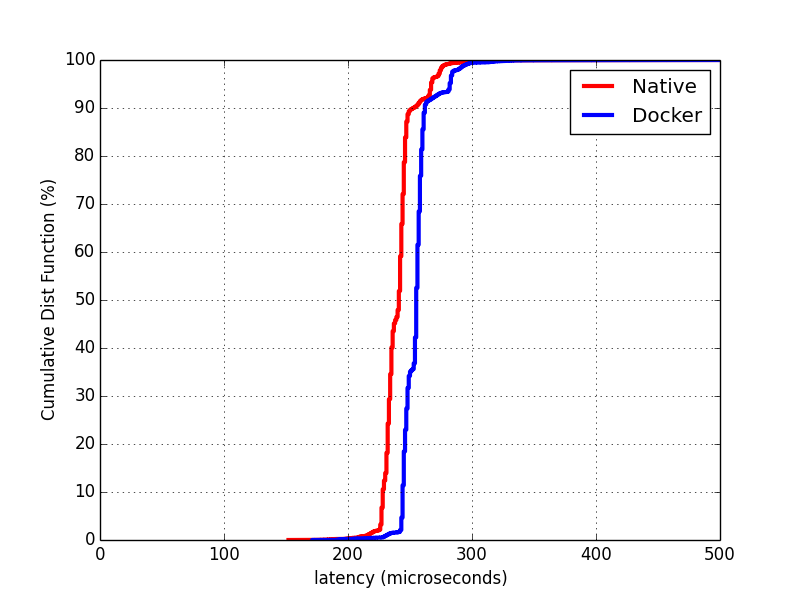
\includegraphics[height=2.5in, width=3in]{cpu_cdf.png}
\caption{The CDF of latency using bare metal and Docker container}
\end{figure}

\begin{table}
\label{tbl:cpubase}
\centering
\caption{Latency measurements of bare metal and Docker container}
\begin{tabular}{|l|c|c|c|} \hline
$$& \textbf{mean(us)} & \textbf{median(us)} & \textbf{p99(us)}\\ \hline
\textbf{Bare metal} & 240.7 & 241.0 & 278.0 \\ \hline
\textbf{Docker container} & 255.2 & 255.0 & 295.0 \\ \hline\end{tabular}
\end{table}

\subsubsection{Case 1}

To test whether Docker would have an impact on the latency performance, we run the server process in a Docker container, with `\textbf{--cpuset-cpus=``3''}' set to realize CPU affinity and the `\textbf{--cpu-shares=1024}' as a default value set in CFS scheduler. When `\textbf{--cpu-shares=1024}' is set, assume that two containers have different shares and are running on the same CPU core. Container A has a share of 1024 and container B has a share of 512, if both containers are CPU-intensive, which means that they take almost all the time to do CPU calculation. The CPU time used by container A and container B would be a ratio of 1024 : 512, which is 2 : 1. We run the test for 10 times. Each time 1,000,000 requests are transmitted between client and server. The CDF result is shown as the blue line in Figure \ref{fig:cpucdf}, and the mean, median and $99^{th}$-percentile position of the measurements are also shown in Table \ref{tbl:cpubase}.

From the results drawn from the above two test cases, we might observe that when using Docker, the CPU latency almost shares the same CDF curve as using bare metal, except a little bias showing an additional fixed amount cost for CPU. Comparing both from the $99^{th}$-percentile column in Table \ref{tbl:cpubase} and the CDF curves in \ref{fig:cpucdf}, Docker container does not have a significant impact on the tail latency performance. Just like mentioned in the report of IBM, Docker containers do have several degradation concerning CPU performance. However, the performance degradation is very low, 4\% in IBM's report about throughput and about 6\% about the mean, median, and $99^{th}$-percentile performance in our research. We might conclude that when running a CPU-intensive application in a Docker container, the performance effect would be very small. Unlike virtual machines, which use hardware-level virtualization technology, Docker container's instructions do not need to be emulated by VMM. However, Docker containers share the same Linux kernel and use the same instructions as the host machine. An x86 instruction might need to be translated to several instructions to run on an ARM CPU. With the help of equation \ref{eq:vmsv} \cite{menasce2005virtualization}, we can do a rough calculation of the virtualization slowdown, where $f_p$ stands for the fraction of privileged instructions executed by a VM and $N_e$ stands for the average number of instructions required by the VMM to emulate a privileged instruction. The reason why Docker containers bring about a slightly slowdown is because when performing CPU isolation, the kernel needs to first check the namespace of the running process, thus the additional instructions would cause the extra latency.

\begin{equation}
\label{eq:vmsv}
S_v = f_p \times N_e + (1 - f_p)
\end{equation}

\subsubsection{Case 2}

Apart from `\textbf{--cpu-shares}', there exist other parameters to limit the resource usage of CPU. `\textbf{--cpu-period}' means the period for the processes in the Docker container to be scheduled on the CPU. It is often used together with the `\textbf{--cpu-quota}'  parameter. The unit of these two parameters are both microseconds. When these parameters are set, it means that processes in the container can use no more than `\textbf{--cpu-quota}' time during each `\textbf{--cpu-period}' time duration. To test whether these two parameters would have a same side effect as `\textbf{--cpu-shares}' that when only one container is assigned to a CPU core, it can take all the cycles of that CPU, we carry out the following experiment:

\begin{table*}
\centering
\caption{Measurements using `\textbf{--cpu-period}' and `\textbf{--cpu-quota}'}
\begin{tabular}{|r|r|r|r|r|r|} \hline
\textbf{quota(us)} & \textbf{mean(us)} & \textbf{median(us)} & \textbf{p99(us)} & \textbf{\# $>$ 1,000us} & \textbf{\# $\times$ quota}\\ \hline
\textbf{1000} & 1035.4 & 307.0 & 7556.0 & 104996 & 104996000\\ \hline
\textbf{1500} & 579.5 & 258.0 & 5816.0 & 68221 & 102331500\\ \hline
\textbf{2000} & 489.0 & 281.0 & 4765.0 & 50187 & 100374000\\ \hline
\textbf{2500} & 361.7 & 260.0 & 3232.0 & 37334 & 93335000\\ \hline
\textbf{3000} & 291.9 & 259.0 & 1741.0 & 14273 & 42819000\\ \hline
\textbf{4000} & 258.0 & 253.0 & 331.0 & 39 & 156000\\ \hline
\textbf{5000} & 263.2 & 255.0 & 341.0 & 0 & 0\\ \hline
\textbf{7000} & 256.7 & 250.0 & 341.0 & 0 & 0\\ \hline
\textbf{10000} & 262.6 & 255.0 & 333.0 & 0 & 0\\ \hline
\end{tabular}
\label{tbl:cpuperiod}
\end{table*}

We first fix `\textbf{--cpu-period=10000}' and vary the value of `\textbf{--cpu-quota}' to see the relationship between these two parameters. We choose values 1,000, 1,500, 2,000, 2,500, 3,000, 4,000, 5,000, 7,000, 10,000 for `\textbf{--cpu-quota}' and observe the results. The reason why we choose these parameters is because the minimum value of both these parameters are 1,000, and if their difference is two large, the measurements might be affected and hard to reach the conclusion. For each test, it is performed for 1,000,000 requests. We measure mean, median, $99^{th}$-percentile of the latencies. We also take the number of requests whose latency is greater than 1,000 us, the minimum time slice, into consideration. The results are shown in Table \ref{tbl:cpuperiod}. 

From Table \ref{tbl:cpuperiod}, we might observe that the latency is increasing incredibly when CPU quota only counts for a small ratio of the total CPU period. From the quota 1000 to 4000, all mean, median and $99^{th}$-percentile are decreasing and the number of test cases whose latency is greater than 1,000 us is also decreasing. Figure \ref{fig:cpuquo} also show the relationship between `\textbf{--cpu-quota}' and the number of requests whose latency is greater than 1,000 us. From this picture, we can see that the number first drops fast and then slowly as quota increases. When quota reaches over 3,000 us, latency suddenly drops fast and finally go to about zero at 4,000.

We make the following guess about the above phenomenon. Unlike using CPU share, once only a single process is using the CPU, it can take all the CPU resources, using CPU period together with CPU quota options will have a force cut off when the CPU usage is over the limited number. Since the client is calling the server continuously, once a request has finished, another request will immediately follows. If the server process has used up its quota during one period, it will sure to give up the CPU and wait until the next period comes. This would cause a very long tail latency in real time services, which is shown as a sudden rise in the $99^{th}$-percentile. Once the service is CPU intensive or being visited quickly, it will add unwilling latency to the service, thus reducing the overall performance.

To prove our guess, we first compute the last column in Table \ref{tbl:cpuperiod}. Assume we need in total time $t_{cpu}$ to do all the computation, which means that the total time the process is running on the CPU. The cpu quota is $t_q$, and the cpu period is $t_p$. The total number of requests blocked by the cpu option $n$ is computed as follows: $n = t_{cpu} \div t_q$. Thus, total time $t_{total}$ needed to compute all the requests is: $t_{total} = n \times t_p$. So once $t_{cpu}$ is determined, we can see that $n \times t_p = t_{cpu}$ is also determined. In our experiment, we assume the cpu time cost for each request is $t_{request}$, and the total number of requests is $r$. So we may see that $t_{cpu} = t_{request} \times r$ is determined. So $n \times t_q$ must be also determined. Which is shown in our experiment as the last column. We can observe that for the case 1000, 1500, 2000, 2500, the product are around 100,000,000, which satisfy our formula. However, we $t_q$ comes to over 3000, the product falls incredibly. This phenomenon occurs because at this time, $t_q$ is greater than the overall CPU used. We use \textit{htop} command to measure CPU usage and the CPU use rate of that CPU is around 30\%. This is the reason why it suddenly falls at the 3000 point, which has $3000 / 10000 = 30\%$, and then quickly goes to 0. We also see from Figure \ref{fig:cpuquo} that when it comes to over 4000, the mean, median and  $99^{th}$-percentile are almost not affected, which means that when the CPU usage of the application is less than the ratio of quota to period, it has low impact on the latency performance.

\begin{figure}
\label{fig:cpuquo}
\centering
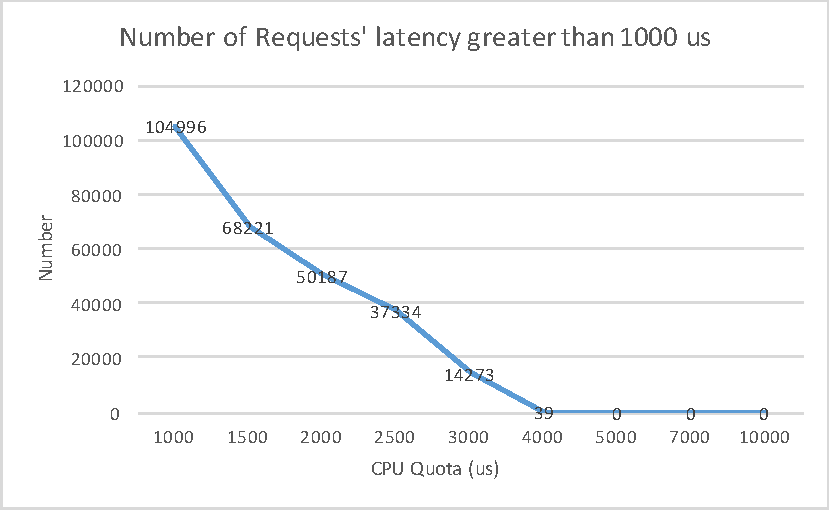
\includegraphics[height=2in, width=2.5in]{cpu_quota.pdf}
\caption{Number of requests' latency greater than 1000 us}
\end{figure}

\subsection{Network Isolation}

In this experiment, server side will send or receive various length data to or from client side. This is done by client calling the server with various length string parameter while server returns nothing. We choose message sizes 1KB, 10KB, 30KB, 50KB, 70KB, 100KB.  These message sizes are chosen as the standard web message sizes from \textit{SPECWeb2009} \cite{specweb2009commerce}. For each experiment, there are 1,000,000 requests.

Sever is hosted in a Docker container on one machine and client is running natively on another machine. Both server and client are assigned to a dedicated CPU to reduce performance interference. We compare two Docker configurations, the first one is to use `\textbf{--net=host}', which means the container directly use the host network port and the network isolation mechanism is not working. The second one is to use the first one is to use `\textbf{-p portA:portB}', which means container uses Linux bridge to communicate to the outside world. It has its own IP address different from the one own by host machine. The \textbf{portA} used by the container is mapped to \textbf{portB} of the host machine, and it is working very similar to the $NAT$ mechanism \cite{tsirtsis2000network}.

\subsubsection{Case 1: Server Receive Data}

In this case, the client is sending data to the server using RPC calls and pass data through string parameters. We compare the mean, median and $99^{th}$-percentile result between using `\textbf{--net=host}' and `\textbf{-p portA:portB}'. The results are shown in Figure \ref{fig:recv}(a-c).

\begin{figure*} 
  \centering 
  \subfigure[Receive: Mean]{ 
    \label{fig:recva} %% label for first subfigure 
    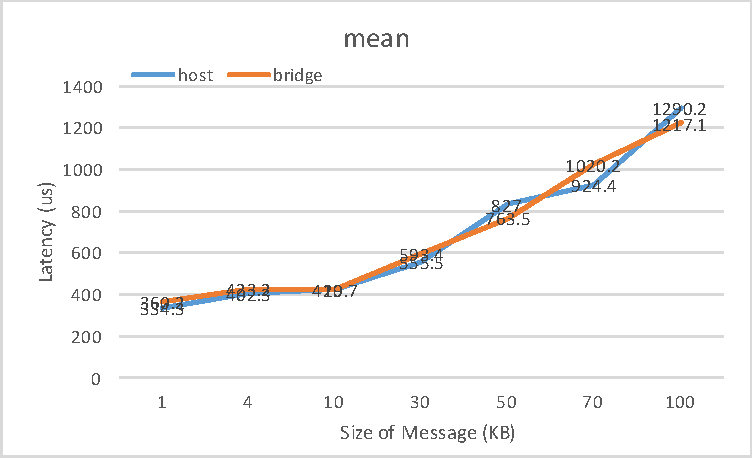
\includegraphics[width=2.2in,height=2.0in]{recv_a.pdf}} 
  %\hspace{0.3in} 
  \subfigure[Receive: Median]{ 
    \label{fig:recvb} %% label for second subfigure 
    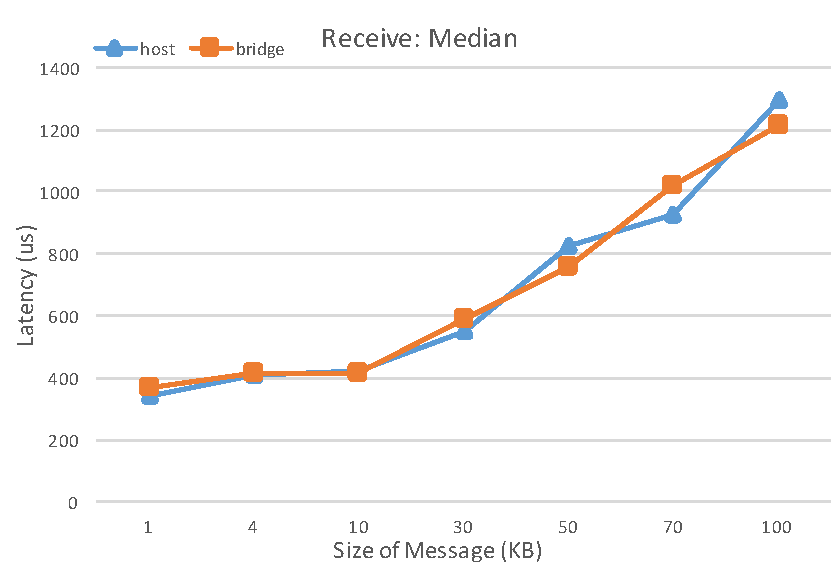
\includegraphics[width=2.2in,height=2.0in]{recv_b.pdf}} 
  %\hspace{0.3in} 
  \subfigure[Receive: $99^{th}$-percentile]{ 
    \label{fig:recvc} %% label for second subfigure 
    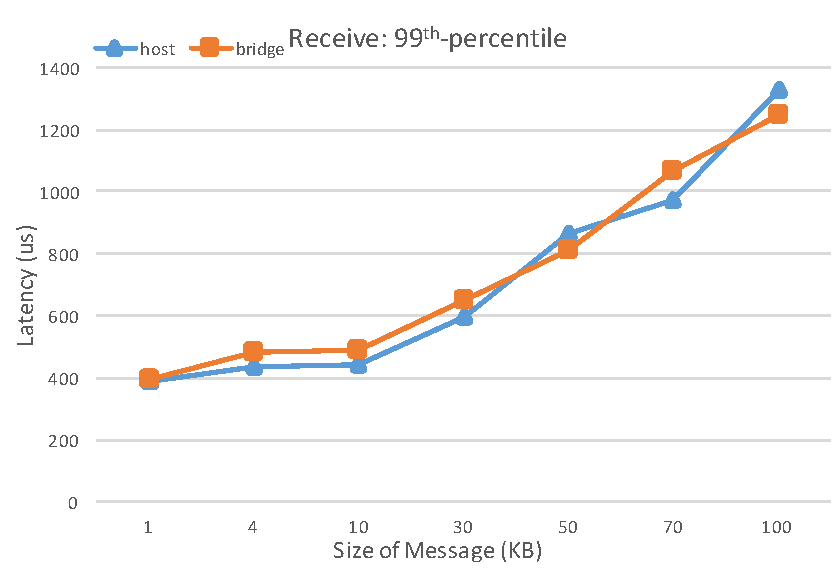
\includegraphics[width=2.2in,height=2.0in]{recv_c.pdf}} 
    \subfigure[Send: Mean]{ 
    \label{fig:senda} %% label for first subfigure 
    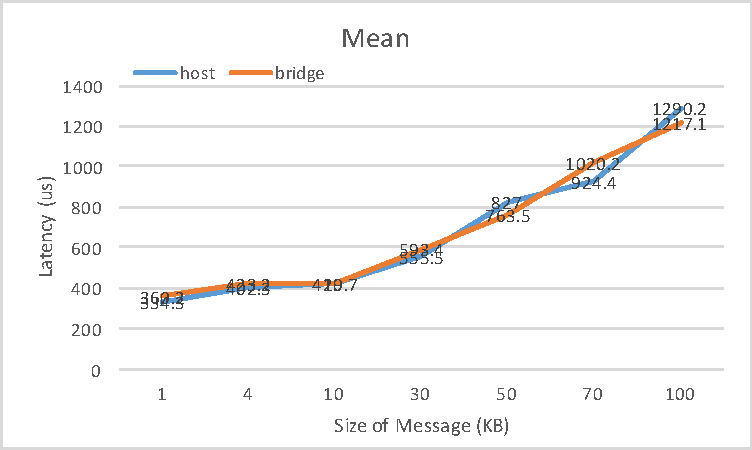
\includegraphics[width=2.2in,height=2.0in]{send_a.pdf}} 
  %\hspace{0.3in} 
  \subfigure[Send: Median]{ 
    \label{fig:sendb} %% label for second subfigure 
    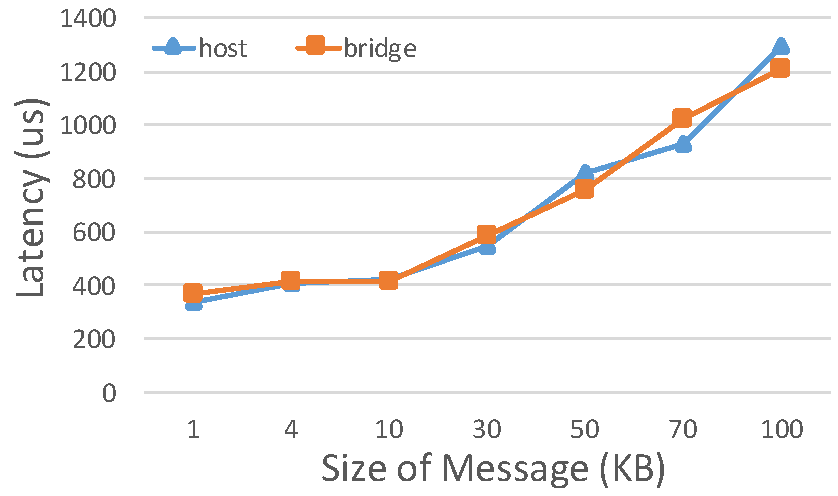
\includegraphics[width=2.2in,height=2.0in]{send_b.pdf}} 
  %\hspace{0.3in} 
  \subfigure[Send: $99^{th}$-percentile]{ 
    \label{fig:sendc} %% label for second subfigure 
    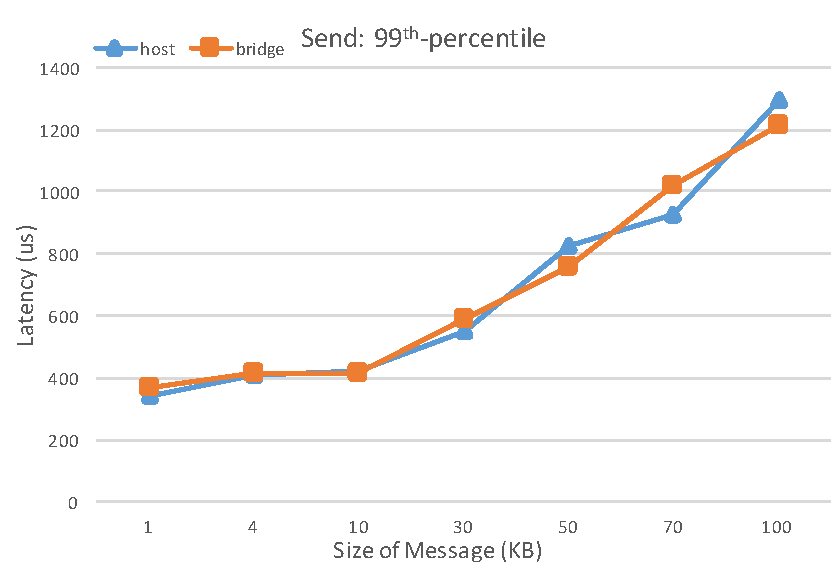
\includegraphics[width=2.2in,height=2.0in]{send_c.pdf}} 
  \caption{Mean, median, and $99^{th}$-percentile latency when server receive and send data.} 
  \label{fig:recv} %% label for entire figure 
\end{figure*}

\subsubsection{Case 2: Server Send Data}

In this case, the client is calling server with a single parameter indicating size and server is returning the corresponding size string. We compare the mean, median and $99^{th}$-percentile result between using `\textbf{--net=host}' and `\textbf{-p portA:portB}'. The results are shown in Figure \ref{fig:recv}(d-f).

\subsubsection{Analysis}

As are shown in both figures, most of the latency using `\textbf{-p portA:portB}' is no more than 110\% of the latency using `\textbf{--net=host}' according to each size group. In fact, when the file size becomes much larger, the result might be very close to each other, and the slowdown percentage is much close to zero. Some of the comparison group even shows a phenomenon where Docker bridge performs better than Docker host. We explain this situation as being caused by the random vibration. This is because many other factors would cause the latency to change slightly, including CPU scheduling, preempting, network contend, and so on. These are not the parts should be talked about in our experiment.

However, IBM's report shows that there is a 80\% slowdown using Docker bridge. So why our experiment draws a totally different result from IBM's research? I think there are several reasons to explain this. First, from our observe of the experiment, we might think the digression is a `one-time degradation'. Which means that it only add a fix amount of latency to each transaction. In our experiment, when the size of the message is small, the impact of this fix amount of latency is very large -- nearly 10\%. However, when the message size becomes much larger, the impact of this latency is negligible, and the random vibration might be the dominant reason of the difference.

In IBM's report, it used docker on both server and client side, which means the messages have gone through the bridge four times, each side two times. While in our experiment, it only happens at server side and total two times. IBM's report uses 100B and 200B message size, while the messages used in our experiment are much larger. Also, we use python and Thrift, which add much extra interference to the CPU and network performance, so the baseline might be much larger than IBM's report. The size 0 situation is over 200 us as shown in previous experiment section. While the latency in IBM's report is less than 100us. So we can not simply describe the impact of Docker bridge on the network performance as a percentage slowdown. It is more like a fix-length degradation.

So where does this fix-size degradation come from? We dive into the source code of Linux bridge to see where this happens. Let us choose the receive stage as an example. When a message has arrived at the NIC, it is uploaded to the upper layer in the network stack. It will first check whether this message is used by more than one application or will it be multicasted. If not, it will not do any process including large amount of data copy. If so, the message will be copied several times and then send to each receiver, thus cost huge amount of extra latency. However, apparently in our experiment and IBM?s experiment, the message is only used by a single application, so there is no process of copying the message. Also, the message transmission is done by transferring a pointer to the message. So these extra functions will only cause a fix amount of extra time. This is why it affect so much in IBM?s report while in ours slightly.

\subsection{File Operations Using AUFS}

Many applications like SQL server and Hadoop might involve disk I/O operations. Disk operation latency of Docker container is thus another issue we should care about. In this experiment, we will not employ a client-server structure. Instead, only one application is hosted in a Docker container. The application will continuously write content of different sizes to a file. The length written each time are 1KB, 4KB, 10KB, 30KB, 50KB, 70kB, 100KB. We will compare two situations, the first one is to directly write messages inside the container, while the second is to write message to a file outside and mounted to the container using `\textbf{-v}' option. To make sure that the message are written to the disk immediately instead of staying in the cache area, each time we write a single message, we will use the `\textbf{flush()}' function to force the message flushed onto the disk. In each experiment group, the application will continuously write 10,000 times and we repeat this operation for 10 times. We will only discuss about the write case instead of the read case to avoid the pre-read situation where blocks of files are read in advance. We note down the mean, median and $99^{th}$-percentile measurements. The results are shown in Figure \ref{fig:write}.

\begin{figure*} 
  \centering 
  \subfigure[Mean]{ 
    \label{fig:recva} %% label for first subfigure 
    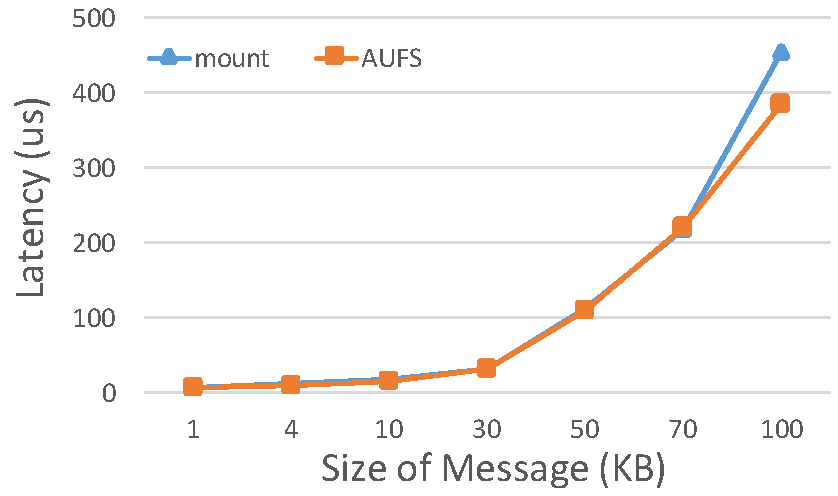
\includegraphics[width=2.2in,height=2.0in]{write_a.pdf}} 
  %\hspace{0.3in} 
  \subfigure[Median]{ 
    \label{fig:recvb} %% label for second subfigure 
    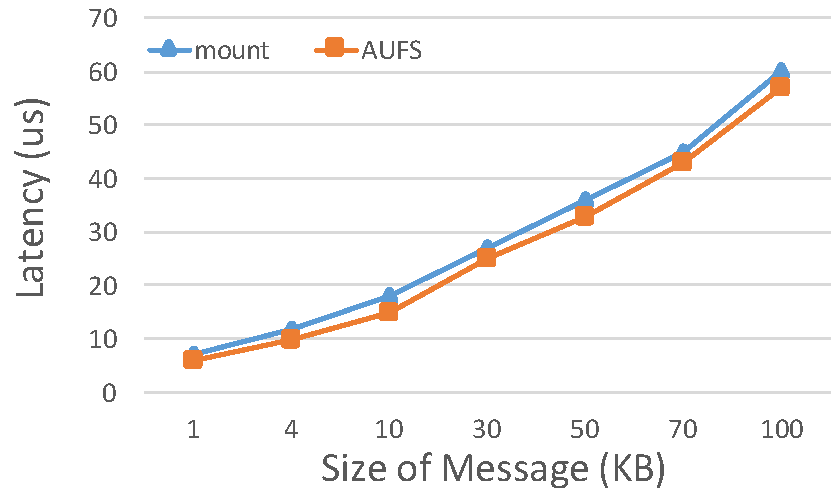
\includegraphics[width=2.2in,height=2.0in]{write_b.pdf}} 
  %\hspace{0.3in} 
  \subfigure[$99^{th}$-percentile]{ 
    \label{fig:recvc} %% label for second subfigure 
    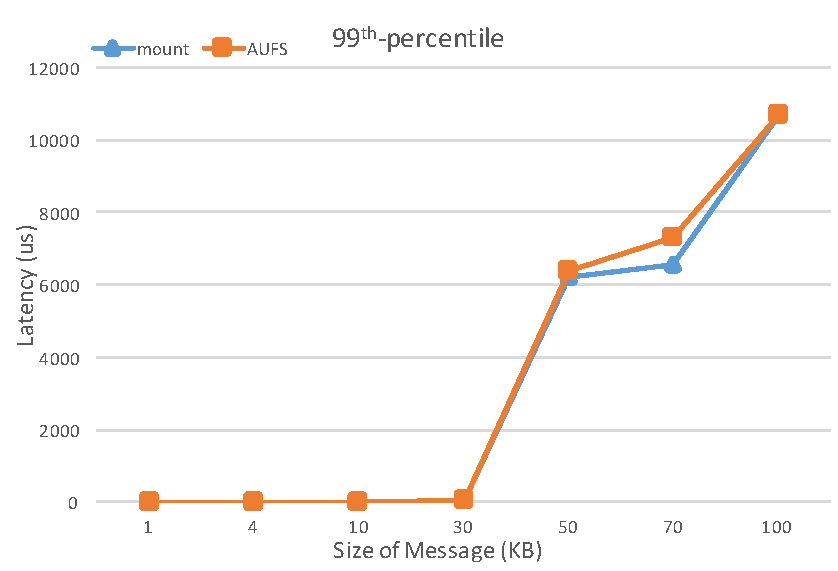
\includegraphics[width=2.2in,height=2.0in]{write_c.pdf}} 
  \caption{Mean, median, and $99^{th}$-percentile file write latency using mount and AUFS.} 
  \label{fig:write} %% label for entire figure 
\end{figure*}

From Figure \ref{fig:write}, we might observe that there is almost no impact on performance using AUFS. This result is the same as the one drawn from IBM's disk I/O report. This phenomenon may be explained as follows. When a file is open, due to the copy-on-write feature of AUFS, a new file is created to hide the original file and a pointer to this file is returned to the application. The following operations are just like the normal operations on a disk file, and there is no fix-length latency degradation as in the network case.

However, there are cases reported that operating on files might involve a significant performance degradation. Considering the feature of AUFS, we guess that the latency lies in the operation of opening a file. To confirm our guess, we carry out another group of experiment where the application continuously open and close a file 1,000,000 times. We note down the time required to open the file and the comparison is shown in Figure \ref{fig:open}.

\begin{figure}
\label{fig:open}
\centering
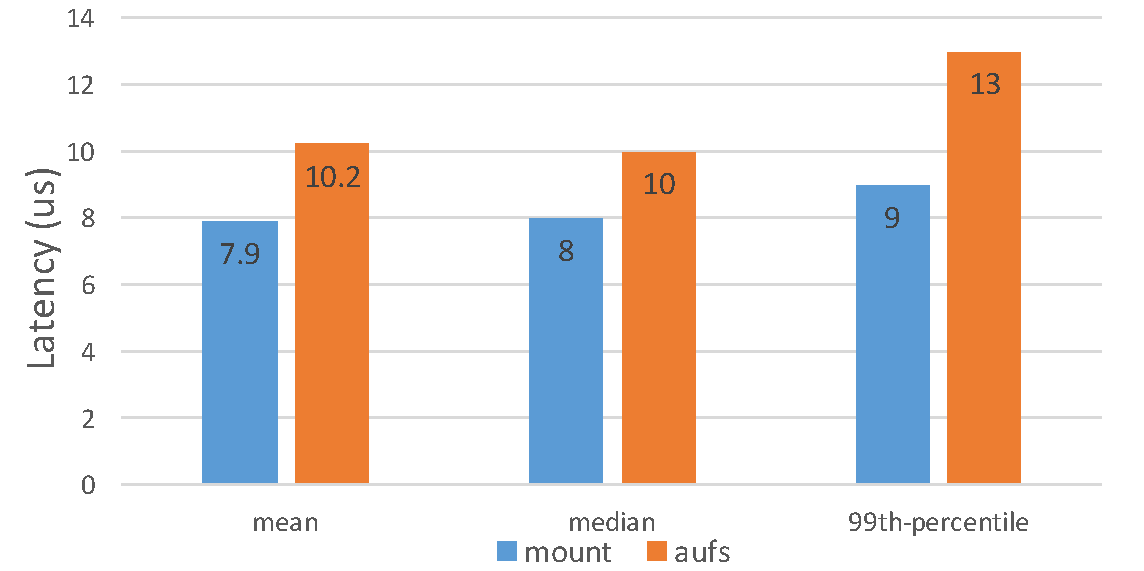
\includegraphics[height=2.5in, width=3in]{open.pdf}
\caption{Latency Comparison between mount and AUFS when opening a file}
\end{figure}

From Figure \ref{fig:open}, we might find there is a huge difference between using mount and AUFS concerning the open time of a file. This is because when using AUFS, since a docker container is implemented using several layers together, it must perform several additional functions to decide which layer the file is in. Sometimes it even has to copy another version of an existing file to perform the copy-on-write operation. These costs might be huge compared to the time to open a file on the bare metal. Also, when first time writing to an existing file in the container, the larger the original file is, the longer the operation latency will be, which is caused by the cost of copy-on-write feature.

\subsection{Increasing AUFS Layers}

Building an image over another is a very convenient feature of Docker. You can simply add some files or run `\textbf{apt get}' command to install applications to the new image. All modifications are done in a new copy-on-write layer based on the original image layers. If a new file share the same name as an existing file, the original file will be hidden and only the newly added file can be seen by user. 

We have observed in the last section that there is no performance slowdown when operating on an opened file. However, the open operation would take extra time due to locating the file in multiple layers and the cost of creating a new copy-on-write layer. Since it might require extra time to locate files in all layers, we guess that when traversing a directory that has many layers, it might go through almost every hidden files in each layer instead of just the visible files.

\begin{figure}
\label{fig:layer}
\centering
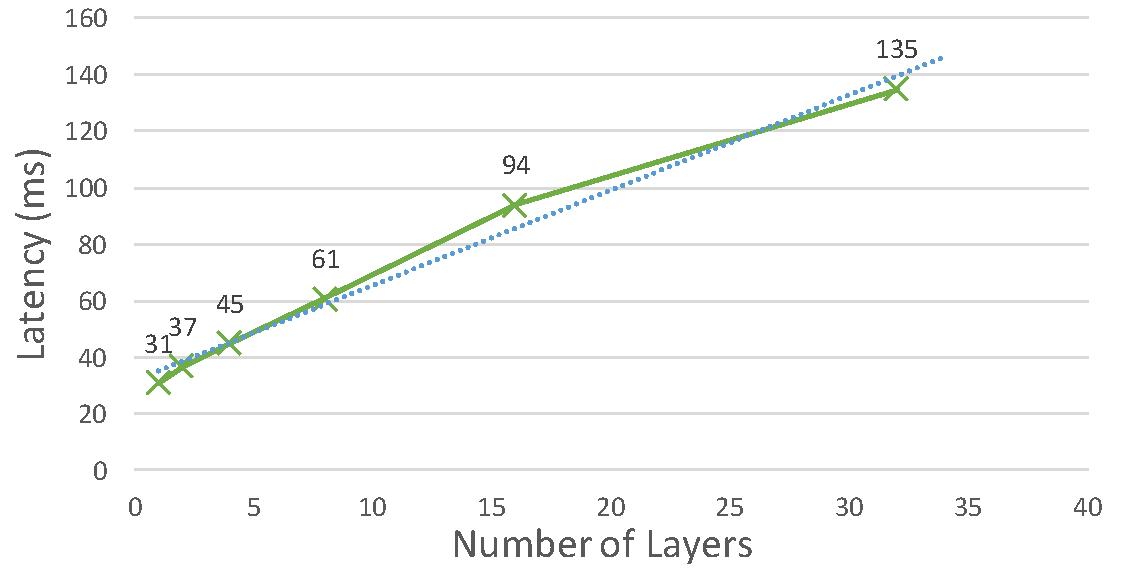
\includegraphics[height=2.5in, width=3in]{layer.pdf}
\caption{\textbf{ls -R} latency measurement}
\end{figure}

To prove our guess, we build images from the official \textbf{ubuntu} image. Each time we build a new image, we add linux kernel source code directory (53.9MB) to the \textbf{/home} directory of the previous image. We build 32 such images, each has a new linux kernel source code directory located in \textbf{/home} hiding the original directory. In each directory, we run the `\textbf{time ls -R /home > > /dev/null}' command to note down the time consumption. Each experiment is done 100 times and we choose the mean measurement of the results. The output are shown in Figure \ref{fig:layer}. It is easy to observe from the figure that with the increment of the number of layers, latency is increasing too. Also, the line is almost linear except for some vibration. This might because the \textbf{ls -R} command will go through each layer of the \textbf{/home} directory. The reason why intercept is not zero is because the additional cost of output messages to \textbf{/dev/null} and there are branch cut in each scan of the hidden layer to avoid too much additional time consumption.





\section{Related Works}

Several institutions and researchers have published related performance tests about Docker. Most of them are about throughput, while a few are concerned with latency. Eder \cite{jbossAnzhuangyupeizhi} did a very simple work using kernel bypass \cite{liu2006high}. He concluded that applications running in a container does not have a obvious impact on its network latency performance. He used \textit{OpenOnload} together with \textit{netperf} to realize the bypass. The results are shown and compared with their average, mean and $99^{th}$-percentile round trip latency. From that report, he concluded that there are almost no performance degradation using Docker container. However, this test might only suitable for private Docker cloud but not public Docker cloud. This is because kernel bypass requires direct access to NIC, which might cause secure problems in public cloud since one can modify the content of other containers as long as they will. However, in private docker cloud, kernel bypass can be a very good choice. Conventionally, once a packet is sent, it has to gone through user space, kernel space and finally arrive at the NIC. With kernel bypass, the packet can directly sent from user space to NIC, which might save some time.

The famous IBM report \cite{felter2015updated} infers that Docker container has a significant impact on overall network performance. The report uses \textit{nuttcp} to measure throughput and also \textit{netperf} to gauge latency. The report shows that there is a over 80\% digression on network round trip latency and also consumes more cpu cycles transferring a single byte using Docker container than native. So why there exists such a big difference between Eder's work and IBM's report? The key point might lies in the fact that one uses kernel bypass while the other doesn't. Using kernel bypass in a Docker container might lead to shorter latency than Docker bridge or Docker host without latency and even faster than bare metal without kernel bypass. From the public cloud perspective, since it is not allowed for customers to use kernel bypass due to security reasons \cite{dua2014virtualization}, IBM's work might be more valuable in this case. However, IBM's report only uses a single group of comparison. It doesn't incorporate more comparison groups to further develop the relationship between round trip latency and other variables like the size of each packet transmitted. 

\section{Conclusion}

Docker might not be so real time latency-friendly. When using the CPU settings, although \textbf{--cpu-shares} might be a good choice since it will not cause a huge tail latency. In public cloud, you have to use a CPU to share multiple applications, using CPU shares will let a single application consumes more CPU than it is allowed to use when other applications are not running on this CPU. This is good for the consumers, but not fair since a consumer enjoys more resource than he has paid. Also, when service providers continuously allocate and deallocate containers on that CPU, applications running on that CPU will gone through a large performance vibration. While using \textbf{--cpu-quota}, it is a good choice for those CPU intensive works like many scientific workflow and HPC applications \cite{xavier2013performance}, but not those real time works due to the possible long tail latency. 

Since the Linux scheduler has two kinds of scheduling algorithms, one is real time \cite{sha2004real} and the other is CFS \cite{jones2009inside}. Docker assumes that users traditionally run applications on a desktop version of Linux, and thus enable the CFS while disable the real time one. There are two way to let the servers have this additional real-time feature. The first one might be to add options for Docker to support to real-time scheduling. The other might be more difficult but will bring a lot good -- implement another scheduling that takes both throughput and real time performance into consideration. And we will not need to reboot the machine to change the setting of CPU scheduler.

Many applications involve small size of messages, like Redis Cache \cite{zawodny2009redis} and NoSQL databases \cite{strauch2011nosql} . When using Docker bridge to transmit message, it will take much more additional time due to their short message size and high throughput, thus reducing the overall performance. But for applications like web gallery, since a photo is usually more than 1MB, the fix-size latency slowdown might be overwhelmed by the system vibration, thus being less important in these cases. When using Linux bridge together with small size messages, it might not be so friendly since the extra consumption is relatively large. We hope that a new method of transmitting information between Docker containers on different machines implemented to reduce this overall latency.

Some applications include many file operations. If the application simply open several big files one time and continuously operate on them, then we can neglect the disk I/O overhead since operating an open file using AUFS is just like operating an open file natively. However, if the application involves huge number of file open operations, it might cause a huge extra latency (over 20\%). So applications running in Docker should not incorporate too many open operations and sometimes the design of the application might have to be changed to suit Docker, thus bringing the programmers a lot of trouble.

Another thing we should bare in mind when using Docker is to reduce overall layers. Some operations like traversing the file system might involve going through hidden files in the low layers of the AUFS. However, we may not need these additional cost since they are totally useless. One way to avoid this is to merge the different layers together and delete unnecessary files, either at container start time or image build time. Then no needless files would be found when traversing the file system.

%\section{Not Mine}
%
%The \textit{proceedings} are the records of a conference.
%ACM seeks to give these conference by-products a uniform,
%high-quality appearance.  To do this, ACM has some rigid
%requirements for the format of the proceedings documents: there
%is a specified format (balanced  double columns), a specified
%set of fonts (Arial or Helvetica and Times Roman) in
%certain specified sizes (for instance, 9 point for body copy),
%a specified live area (18 $\times$ 23.5 cm [7" $\times$ 9.25"]) centered on
%the page, specified size of margins (1.9 cm [0.75"]) top, (2.54 cm [1"]) bottom
%and (1.9 cm [.75"]) left and right; specified column width
%(8.45 cm [3.33"]) and gutter size (.83 cm [.33"]).
%
%The good news is, with only a handful of manual
%settings\footnote{Two of these, the {\texttt{\char'134 numberofauthors}}
%and {\texttt{\char'134 alignauthor}} commands, you have
%already used; another, {\texttt{\char'134 balancecolumns}}, will
%be used in your very last run of \LaTeX\ to ensure
%balanced column heights on the last page.}, the \LaTeX\ document
%class file handles all of this for you.
%
%The remainder of this document is concerned with showing, in
%the context of an ``actual'' document, the \LaTeX\ commands
%specifically available for denoting the structure of a
%proceedings paper, rather than with giving rigorous descriptions
%or explanations of such commands.
%
%\section{The {\secit Body} of The Paper}
%Typically, the body of a paper is organized
%into a hierarchical structure, with numbered or unnumbered
%headings for sections, subsections, sub-subsections, and even
%smaller sections.  The command \texttt{{\char'134}section} that
%precedes this paragraph is part of such a
%hierarchy.\footnote{This is the second footnote.  It
%starts a series of three footnotes that add nothing
%informational, but just give an idea of how footnotes work
%and look. It is a wordy one, just so you see
%how a longish one plays out.} \LaTeX\ handles the numbering
%and placement of these headings for you, when you use
%the appropriate heading commands around the titles
%of the headings.  If you want a sub-subsection or
%smaller part to be unnumbered in your output, simply append an
%asterisk to the command name.  Examples of both
%numbered and unnumbered headings will appear throughout the
%balance of this sample document.
%
%Because the entire article is contained in
%the \textbf{document} environment, you can indicate the
%start of a new paragraph with a blank line in your
%input file; that is why this sentence forms a separate paragraph.
%
%\subsection{Type Changes and {\subsecit Special} Characters}
%We have already seen several typeface changes in this sample.  You
%can indicate italicized words or phrases in your text with
%the command \texttt{{\char'134}textit}; emboldening with the
%command \texttt{{\char'134}textbf}
%and typewriter-style (for instance, for computer code) with
%\texttt{{\char'134}texttt}.  But remember, you do not
%have to indicate typestyle changes when such changes are
%part of the \textit{structural} elements of your
%article; for instance, the heading of this subsection will
%be in a sans serif\footnote{A third footnote, here.
%Let's make this a rather short one to
%see how it looks.} typeface, but that is handled by the
%document class file. Take care with the use
%of\footnote{A fourth, and last, footnote.}
%the curly braces in typeface changes; they mark
%the beginning and end of
%the text that is to be in the different typeface.
%
%You can use whatever symbols, accented characters, or
%non-English characters you need anywhere in your document;
%you can find a complete list of what is
%available in the \textit{\LaTeX\
%User's Guide}\cite{Lamport:LaTeX}.
%
%\subsection{Math Equations}
%You may want to display math equations in three distinct styles:
%inline, numbered or non-numbered display.  Each of
%the three are discussed in the next sections.
%
%\subsubsection{Inline (In-text) Equations}
%A formula that appears in the running text is called an
%inline or in-text formula.  It is produced by the
%\textbf{math} environment, which can be
%invoked with the usual \texttt{{\char'134}begin. . .{\char'134}end}
%construction or with the short form \texttt{\$. . .\$}. You
%can use any of the symbols and structures,
%from $\alpha$ to $\omega$, available in
%\LaTeX\cite{Lamport:LaTeX}; this section will simply show a
%few examples of in-text equations in context. Notice how
%this equation: \begin{math}\lim_{n\rightarrow \infty}x=0\end{math},
%set here in in-line math style, looks slightly different when
%set in display style.  (See next section).
%
%\subsubsection{Display Equations}
%A numbered display equation -- one set off by vertical space
%from the text and centered horizontally -- is produced
%by the \textbf{equation} environment. An unnumbered display
%equation is produced by the \textbf{displaymath} environment.
%
%Again, in either environment, you can use any of the symbols
%and structures available in \LaTeX; this section will just
%give a couple of examples of display equations in context.
%First, consider the equation, shown as an inline equation above:
%\begin{equation}\lim_{n\rightarrow \infty}x=0\end{equation}
%Notice how it is formatted somewhat differently in
%the \textbf{displaymath}
%environment.  Now, we'll enter an unnumbered equation:
%\begin{displaymath}\sum_{i=0}^{\infty} x + 1\end{displaymath}
%and follow it with another numbered equation:
%\begin{equation}\sum_{i=0}^{\infty}x_i=\int_{0}^{\pi+2} f\end{equation}
%just to demonstrate \LaTeX's able handling of numbering.
%
%\subsection{Citations}
%Citations to articles \cite{bowman:reasoning,
%clark:pct, braams:babel, herlihy:methodology, soltesz2007container},
%conference proceedings \cite{clark:pct} or
%books \cite{salas:calculus, Lamport:LaTeX} listed
%in the Bibliography section of your
%article will occur throughout the text of your article.
%You should use BibTeX to automatically produce this bibliography;
%you simply need to insert one of several citation commands with
%a key of the item cited in the proper location in
%the \texttt{.tex} file \cite{Lamport:LaTeX}.
%The key is a short reference you invent to uniquely
%identify each work; in this sample document, the key is
%the first author's surname and a
%word from the title.  This identifying key is included
%with each item in the \texttt{.bib} file for your article.
%
%The details of the construction of the \texttt{.bib} file
%are beyond the scope of this sample document, but more
%information can be found in the \textit{Author's Guide},
%and exhaustive details in the \textit{\LaTeX\ User's
%Guide}\cite{Lamport:LaTeX}.
%
%This article shows only the plainest form
%of the citation command, using \texttt{{\char'134}cite}.
%This is what is stipulated in the SIGS style specifications.
%No other citation format is endorsed or supported.
%
%\subsection{Tables}
%Because tables cannot be split across pages, the best
%placement for them is typically the top of the page
%nearest their initial cite.  To
%ensure this proper ``floating'' placement of tables, use the
%environment \textbf{table} to enclose the table's contents and
%the table caption.  The contents of the table itself must go
%in the \textbf{tabular} environment, to
%be aligned properly in rows and columns, with the desired
%horizontal and vertical rules.  Again, detailed instructions
%on \textbf{tabular} material
%is found in the \textit{\LaTeX\ User's Guide}.
%
%Immediately following this sentence is the point at which
%Table 1 is included in the input file; compare the
%placement of the table here with the table in the printed
%dvi output of this document.
%
%\begin{table}
%\centering
%\caption{Frequency of Special Characters}
%\begin{tabular}{|c|c|l|} \hline
%Non-English or Math&Frequency&Comments\\ \hline
%\O & 1 in 1,000& For Swedish names\\ \hline
%$\pi$ & 1 in 5& Common in math\\ \hline
%\$ & 4 in 5 & Used in business\\ \hline
%$\Psi^2_1$ & 1 in 40,000& Unexplained usage\\
%\hline\end{tabular}
%\end{table}
%
%To set a wider table, which takes up the whole width of
%the page's live area, use the environment
%\textbf{table*} to enclose the table's contents and
%the table caption.  As with a single-column table, this wide
%table will ``float" to a location deemed more desirable.
%Immediately following this sentence is the point at which
%Table 2 is included in the input file; again, it is
%instructive to compare the placement of the
%table here with the table in the printed dvi
%output of this document.
%
%
%\begin{table*}
%\centering
%\caption{Some Typical Commands}
%\begin{tabular}{|c|c|l|} \hline
%Command&A Number&Comments\\ \hline
%\texttt{{\char'134}alignauthor} & 100& Author alignment\\ \hline
%\texttt{{\char'134}numberofauthors}& 200& Author enumeration\\ \hline
%\texttt{{\char'134}table}& 300 & For tables\\ \hline
%\texttt{{\char'134}table*}& 400& For wider tables\\ \hline\end{tabular}
%\end{table*}
%% end the environment with {table*}, NOTE not {table}!
%
%\subsection{Figures}
%Like tables, figures cannot be split across pages; the
%best placement for them
%is typically the top or the bottom of the page nearest
%their initial cite.  To ensure this proper ``floating'' placement
%of figures, use the environment
%\textbf{figure} to enclose the figure and its caption.
%
%This sample document contains examples of \textbf{.eps} files to be
%displayable with \LaTeX.  If you work with pdf\LaTeX, use files in the
%\textbf{.pdf} format.  Note that most modern \TeX\ system will convert
%\textbf{.eps} to \textbf{.pdf} for you on the fly.  More details on
%each of these is found in the \textit{Author's Guide}.
%
%\begin{figure}
%\centering
%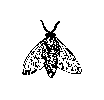
\includegraphics{fly}
%\caption{A sample black and white graphic.}
%\end{figure}
%
%\begin{figure}
%\centering
%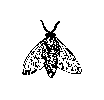
\includegraphics[height=1in, width=1in]{fly}
%\caption{A sample black and white graphic
%that has been resized with the \texttt{includegraphics} command.}
%\end{figure}
%
%
%As was the case with tables, you may want a figure
%that spans two columns.  To do this, and still to
%ensure proper ``floating'' placement of tables, use the environment
%\textbf{figure*} to enclose the figure and its caption.
%and don't forget to end the environment with
%{figure*}, not {figure}!
%
%\begin{figure*}
%\centering
%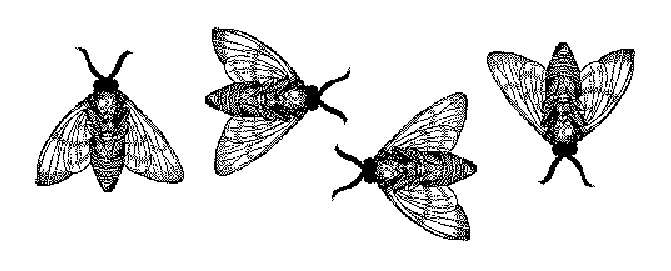
\includegraphics{flies}
%\caption{A sample black and white graphic
%that needs to span two columns of text.}
%\end{figure*}
%
%
%\begin{figure}
%\centering
%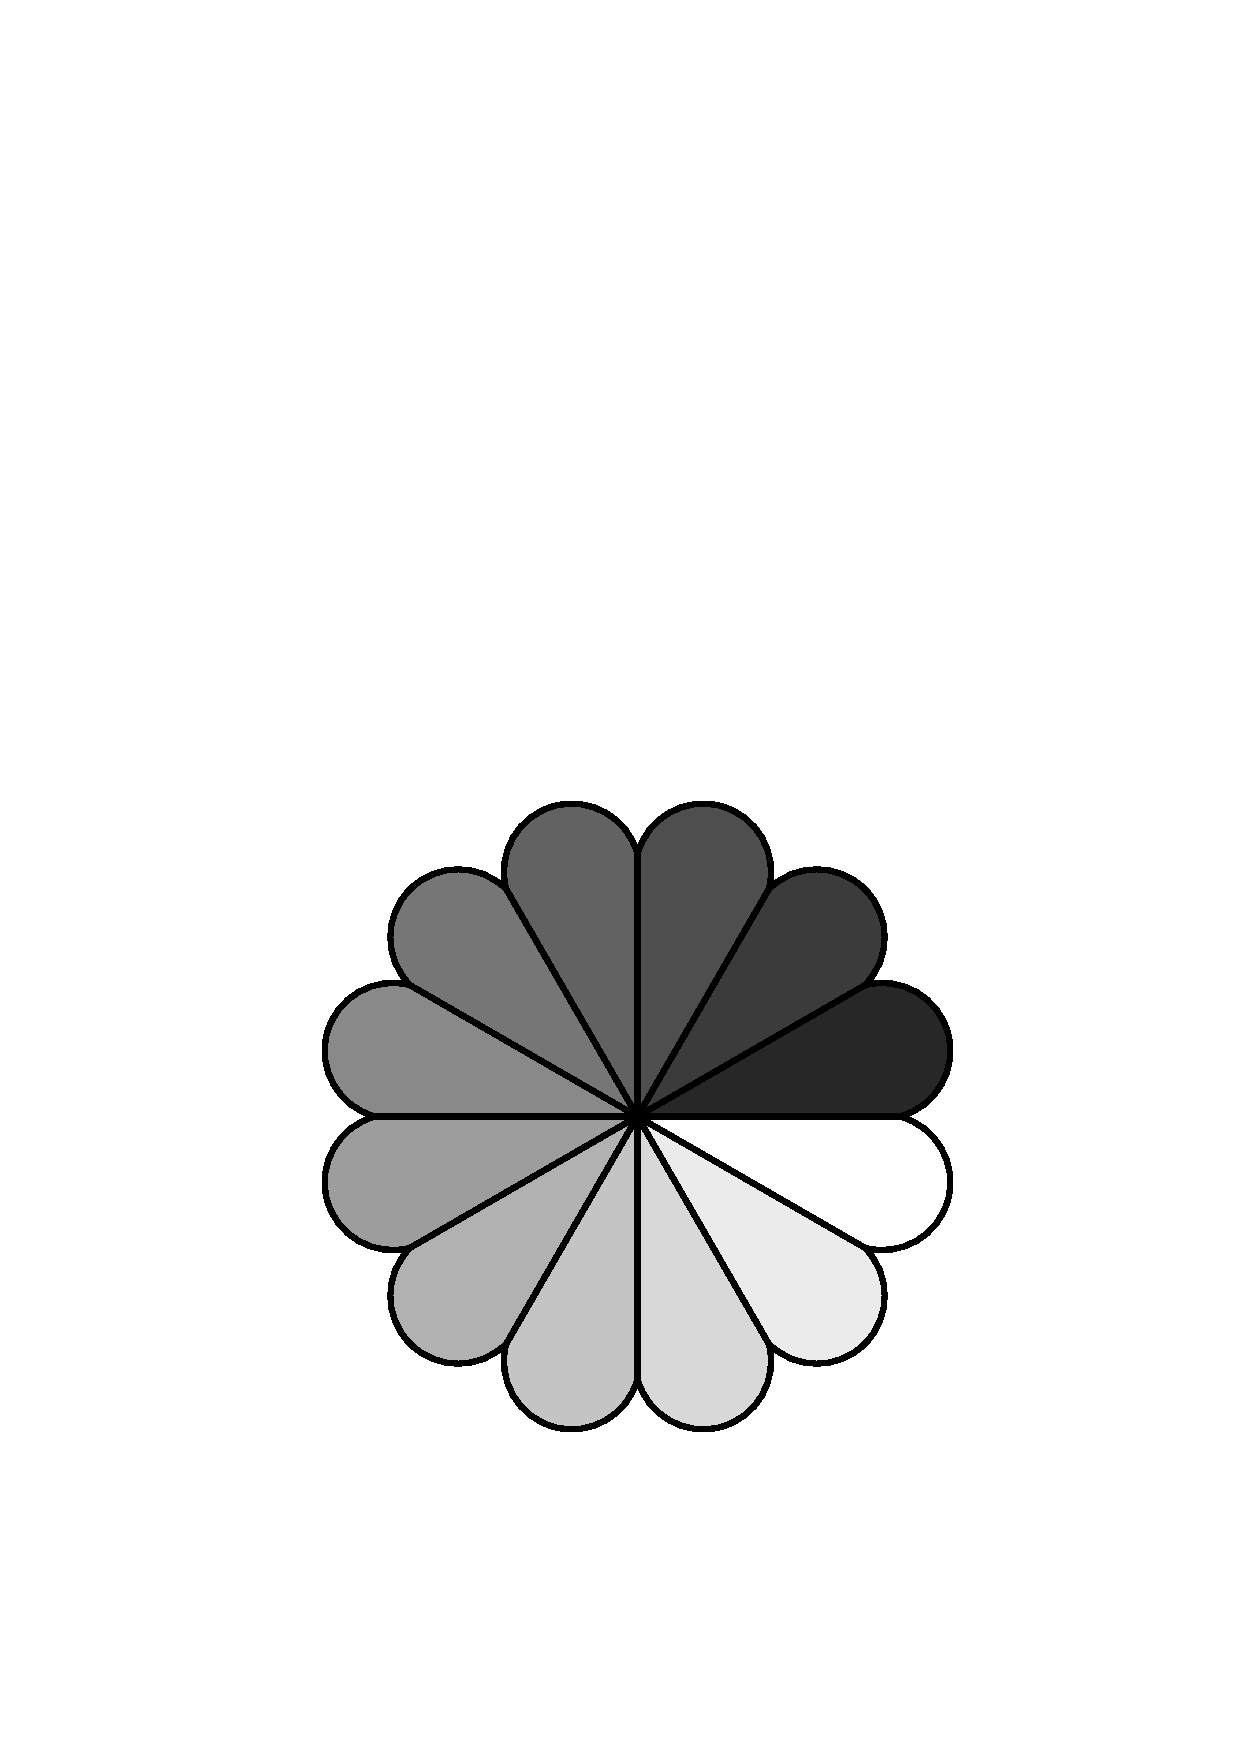
\includegraphics[height=1in, width=1in]{rosette}
%\caption{A sample black and white graphic that has
%been resized with the \texttt{includegraphics} command.}
%\vskip -6pt
%\end{figure}
%
%\subsection{Theorem-like Constructs}
%Other common constructs that may occur in your article are
%the forms for logical constructs like theorems, axioms,
%corollaries and proofs.  There are
%two forms, one produced by the
%command \texttt{{\char'134}newtheorem} and the
%other by the command \texttt{{\char'134}newdef}; perhaps
%the clearest and easiest way to distinguish them is
%to compare the two in the output of this sample document:
%
%This uses the \textbf{theorem} environment, created by
%the\linebreak\texttt{{\char'134}newtheorem} command:
%\newtheorem{theorem}{Theorem}
%\begin{theorem}
%Let $f$ be continuous on $[a,b]$.  If $G$ is
%an antiderivative for $f$ on $[a,b]$, then
%\begin{displaymath}\int^b_af(t)dt = G(b) - G(a).\end{displaymath}
%\end{theorem}
%
%The other uses the \textbf{definition} environment, created
%by the \texttt{{\char'134}newdef} command:
%\newdef{definition}{Definition}
%\begin{definition}
%If $z$ is irrational, then by $e^z$ we mean the
%unique number which has
%logarithm $z$: \begin{displaymath}{\log e^z = z}\end{displaymath}
%\end{definition}
%
%Two lists of constructs that use one of these
%forms is given in the
%\textit{Author's  Guidelines}.
% 
%There is one other similar construct environment, which is
%already set up
%for you; i.e. you must \textit{not} use
%a \texttt{{\char'134}newdef} command to
%create it: the \textbf{proof} environment.  Here
%is a example of its use:
%\begin{proof}
%Suppose on the contrary there exists a real number $L$ such that
%\begin{displaymath}
%\lim_{x\rightarrow\infty} \frac{f(x)}{g(x)} = L.
%\end{displaymath}
%Then
%\begin{displaymath}
%l=\lim_{x\rightarrow c} f(x)
%= \lim_{x\rightarrow c}
%\left[ g{x} \cdot \frac{f(x)}{g(x)} \right ]
%= \lim_{x\rightarrow c} g(x) \cdot \lim_{x\rightarrow c}
%\frac{f(x)}{g(x)} = 0\cdot L = 0,
%\end{displaymath}
%which contradicts our assumption that $l\neq 0$.
%\end{proof}
%
%Complete rules about using these environments and using the
%two different creation commands are in the
%\textit{Author's Guide}; please consult it for more
%detailed instructions.  If you need to use another construct,
%not listed therein, which you want to have the same
%formatting as the Theorem
%or the Definition\cite{salas:calculus} shown above,
%use the \texttt{{\char'134}newtheorem} or the
%\texttt{{\char'134}newdef} command,
%respectively, to create it.
%
%\subsection*{A {\secit Caveat} for the \TeX\ Expert}
%Because you have just been given permission to
%use the \texttt{{\char'134}newdef} command to create a
%new form, you might think you can
%use \TeX's \texttt{{\char'134}def} to create a
%new command: \textit{Please refrain from doing this!}
%Remember that your \LaTeX\ source code is primarily intended
%to create camera-ready copy, but may be converted
%to other forms -- e.g. HTML. If you inadvertently omit
%some or all of the \texttt{{\char'134}def}s recompilation will
%be, to say the least, problematic.
%
%\section{Conclusions}
%This paragraph will end the body of this sample document.
%Remember that you might still have Acknowledgments or
%Appendices; brief samples of these
%follow.  There is still the Bibliography to deal with; and
%we will make a disclaimer about that here: with the exception
%of the reference to the \LaTeX\ book, the citations in
%this paper are to articles which have nothing to
%do with the present subject and are used as
%examples only.
%\end{document}  % This is where a 'short' article might terminate

%ACKNOWLEDGMENTS are optional
%\section{Acknowledgments}
%This section is optional; it is a location for you
%to acknowledge grants, funding, editing assistance and
%what have you.  In the present case, for example, the
%authors would like to thank Gerald Murray of ACM for
%his help in codifying this \textit{Author's Guide}
%and the \textbf{.cls} and \textbf{.tex} files that it describes.

%
% The following two commands are all you need in the
% initial runs of your .tex file to
% produce the bibliography for the citations in your paper.
\bibliographystyle{abbrv}
\bibliography{sigproc}  % sigproc.bib is the name of the Bibliography in this case


% You must have a proper ".bib" file
%  and remember to run:
% latex bibtex latex latex
% to resolve all references
%
% ACM needs 'a single self-contained file'!
%
%APPENDICES are optional
%\balancecolumns
%\appendix
%%Appendix A
%\section{Headings in Appendices}
%The rules about hierarchical headings discussed above for
%the body of the article are different in the appendices.
%In the \textbf{appendix} environment, the command
%\textbf{section} is used to
%indicate the start of each Appendix, with alphabetic order
%designation (i.e. the first is A, the second B, etc.) and
%a title (if you include one).  So, if you need
%hierarchical structure
%\textit{within} an Appendix, start with \textbf{subsection} as the
%highest level. Here is an outline of the body of this
%document in Appendix-appropriate form:
%\subsection{Introduction}
%\subsection{The Body of the Paper}
%\subsubsection{Type Changes and  Special Characters}
%\subsubsection{Math Equations}
%\paragraph{Inline (In-text) Equations}
%\paragraph{Display Equations}
%\subsubsection{Citations}
%\subsubsection{Tables}
%\subsubsection{Figures}
%\subsubsection{Theorem-like Constructs}
%\subsubsection*{A Caveat for the \TeX\ Expert}
%\subsection{Conclusions}
%\subsection{Acknowledgments}
%\subsection{Additional Authors}
%This section is inserted by \LaTeX; you do not insert it.
%You just add the names and information in the
%\texttt{{\char'134}additionalauthors} command at the start
%of the document.
%\subsection{References}
%Generated by bibtex from your ~.bib file.  Run latex,
%then bibtex, then latex twice (to resolve references)
%to create the ~.bbl file.  Insert that ~.bbl file into
%the .tex source file and comment out
%the command \texttt{{\char'134}thebibliography}.
%% This next section command marks the start of
%% Appendix B, and does not continue the present hierarchy
%\section{More Help for the Hardy}
%The sig-alternate.cls file itself is chock-full of succinct
%and helpful comments.  If you consider yourself a moderately
%experienced to expert user of \LaTeX, you may find reading
%it useful but please remember not to change it.
%%\balancecolumns % GM June 2007
%% That's all folks!
\end{document}
